\chapter{Design}

\section{At my Disposal} 

\subsection{Hardware}
The primary hardware requirement is a very large amount of SSD storage. SSD storage can provide us with fast write speeds required to churn through the huge volume of data that must be written to Neo4J for the initial database setup.
\\\\
The hardware the department has at its disposal is a machine named 'satoshi' and has the following specification:
\begin{itemize}
    \item \textbf{Processor}: 24 core AMD EPYC 7401 
    \item \textbf{Memory}: \todo{get machine specification}
\end{itemize}
However, I will be using a VM on this machine, allocated a generous amount of the resource available, but of course not all. Additionally, I have root access on this VM so I am not limited to the software I am able to install on it. 
\\\\
My VM has the following resource allocated to it (initially):
\begin{itemize}
    \item \textbf{Cores}: 16 cores 
    \item \textbf{Memory}: 16GB
    \item \textbf{Storage}: \~5TB SSD Free
\end{itemize}

\subsection{Bitcoin Full Node}
There already exists a Bitcoin Full Node running in a persistent Docker container which I am able to connect to. Using the RPC interface provided by Bitcoin Core, I am able to poll and fetch Bitcoin data. 

\section{Technology Assessment}


\subsection{Graph Databases}
A graph database is a type of database where the relations between data are of equal importance to the data itself. Data does not need to be constricted to a pre-defined structure; rather it is stored using a flexible combination of nodes and relationships between them. 

\subsubsection{Neo4J}
Neo4J is an open-source, NoSQL graph-database providing ACID compliant transactions.

\subsection{Why use a Graph DB for storing Bitcoin?}
Graph DB's provide efficient traversing of nodes; allowing million of connections to be traversed per second per core \cite{RefWorks:doc:5c98f0c6e4b00cbb4da393d8}. Scaling independently to the size of the data-set, a graph database is excellently suited for storing the vast, complex data-set constituting the Bitcoin Blockchain. 


\subsection{Blockchain2graph}
A company Blockchain Inspector who are 'using Artificial Intelligence to fight fraud in the Blockchain' have open-sourced a tool they use with the claim that it extracts Bitcoin data and writes it to a Neo4J database . 

\subsection{Bitcoin to Neo4J Tool}
There exists an open source tool, built by the author of the website \url{learnmeabitcoin.com}, which populates a Neo4J database with the entire Bitcoin Blockchain \cite{RefWorks:doc:5c98e031e4b068320632cef2}. This tool requires a full Bitcoin node to be run in order to have the .dat files stored locally; the tool will parse the .dat files and write them using Cypher queries to the Neo4J database. This approach has the advantage that it is a respected approach in the community to this task and has been cited a number of times by those seeking to achieve the same goal \cite{RefWorks:doc:5c98e0cde4b044512c0b8641}; however, the tool will take several weeks (apparently 60+ days) to complete the import. 

\subsection{Data Lake}
A data lake is an approach to data storage which does not care about format, data can be structured, non-structured or partially structured; it essentially stores data in its raw-format and is often used as a halfway-house for storing data once ingesting data before it is processed and/or analysed. Apache Hadoop is an example of a technology able to host a data lake. There are also cloud hosted technologies, such as Amazon S3 or Microsoft Azure, that are able to provide a similar function. 

\subsection{Approaches}
There exist several approaches to populating a database with the Bitcoin Blockchain; since we are working with a dataset of such vast scale, it is certainly a worthwhile investment at this stage to analyse the merits of each approach and decide which will be most suitable. Otherwise, taking a naive approach would risk a very time consuming, and potentially fragile process, which may hamper progression with subsequent stages of this project. 



\subsubsection{Overview of Approaches}
\begin{enumerate}
    \item Running a full Bitcoin node [see \ref{background-nodes}]. Download the entire Blockchain, use a custom script to parse the files write the data to the database. Keep database up to date using long polling / \gls{rpc}. 
    \item Leverage some of the work done by a previous project in the Department of Computing at Imperial for Blockchain health monitoring \cite{RefWorks:doc:5c6bd151e4b041254f892045}. The initial population of the database would require re-running the RPC approach used in this project, then creating a Kafka consumer to keep the database up to date. 
    \item Combining the two approaches of above: create a custom script for initial database population, but then use the Bitcoin health service for keeping the database up to date. 
\end{enumerate}


\subsection{Neo4J}

\subsubsection{Bulk Import Tool}
Neo4J provides functionality for bulk importing data \cite{RefWorks:doc:5c6ab610e4b02c4a19ae3ed1}. A Neo4J blog describes an example use of this functionality: importing a  vast 66GB dataset from Stackoverflow into a new Neo4J database \cite{RefWorks:doc:5c6ab2bae4b08c9b85da964f}; however, this is less than a third the size of the Bitcoin blockchain (approximately 197GB at the beginning of January 2019 \cite{RefWorks:doc:5c6ab1a3e4b05e3aaec0ffc8}).
\\\\ 
The Stackoverflow import example shows usage of Cypher features for improving the efficiency of bulk imports, such as 'constraints', 'indexes', 'distinct'  in order to make the import more efficient. Another useful feature is periodicc commit' which allows the transaction state to be intermittently committed to storage, and the memory Neo4J is using to hold this state to be flushed. 
\\\\
The import tool is designed to take advantage of the hardware at it's disposal; ideal for our use-case where we have a large amount of SSD and processing power available, and we simply need to ensure we can take full advantage of it. The Stackoverflow import took just over 3 minutes to complete \cite{RefWorks:doc:5c6ab2bae4b08c9b85da964f}. 
\\\\
The constraints of this approach is that it requires the data to be in a CSV format, possibly requiring some conversion of the data format before the import can begin. 

\subsubsection{Memory Recommendations}
Neo4J provides a tool which advises how to configure memory parameters for Neo4J. By passing the command the database and the memory available to Neo4J, it recommends the suggested memory configuration (e.g. heap initial size, max size etc.). 

\subsection{Running a full node}
Running a full node (Bitcoin Core) would download the entire Bitcoin Blockchain to the current tip; the blockchain is currently at ~197GB\cite{RefWorks:doc:5c6ab1a3e4b05e3aaec0ffc8} in size and would consume a considerable amount of storage, and time to download). This would provide the .dat files containing all Bitcoin Blockchain data to the date of download. 


\section{Database Population Approach}
\todo{DRAFT : IMPLEMENTATION} 
There were two main phases to populating the database. The first phase was to fetch historical Bitcoin data from the Genesis block to the present day. 
\begin{itemize}
    \item Plugged into the health monitoring service. Used Flux streams, RPC to fetch the bitcoin data. Then parsed this data and wrote it to CSV files. 
    \item Problem: Duplicates in the address file. Solution: Using GNU's sort -u on the address file, rather than using --ignore-duplicates as this massively slows down the bulk import process
    \item Once the CSV files were generated, the Neo4J bulk import tool could be run, feeding a number of header files, the relationship files and the CSV files containing all of the data. 
    
\end{itemize}

\subsection{Historic Data Population}
An existing project in Java exists to extract historical data from several blockchains and write them to a Neo4J database.\todo{Cite the project} I augmented this project with functionality which performed the fetching of data using parallel WebFlux streams, and wrote the data in a CSV format, rather than to MongoDB. The points below outline the core steps taken to implement the historical population functionality. 

\begin{itemize}
    \item Introduced a new API endpoint for Admin usage. The new endpoint was named \texttt{extractBitcoinToNeo4j}. This accepted two arguments as path variables, \texttt{fromHeight} and \texttt{toHeight} which are to be used to define the range of blocks to fetch data from. 
    \item Using the parameters \texttt{fromHeight} and \texttt{toHeight}, I then generate a Flux stream which uses RPC to invoke the method \texttt{getBlockHash} on a \textit{bitcoind} instance running in a container on the same machine. 
    \item The Flux stream of block hashes are then mapped to the actual block data using flux's \texttt{flatMap} operation and by invoking the method \texttt{getBlock}, passing it the block hash from the previous step. 
    \item The block data is retrieved and deserialized to an intermediary representation in Java. Each block will then be written to a CSV file in the format required for an import into Neo4J. 
    \item The retrieval of a single block will then kick off the process of fetching transactions; the Flux of blocks will be mapped to individual transactions by fetching each of the transaction ID's in the block and again using RPC to invoke the \texttt{getrawtransaction} on the \textit{bitcoind} instance in order to fetch all the data for each transaction. 
    \item Each retrieved transaction will be written to CSV, in addition to writing the relationships between transactions, blocks and outputs to their own CSV files. 
\end{itemize}

\subsection{Data Format}
\subsubsection{Data Nodes}
\begin{itemize}
    \item \texttt{BLOCK} : A Bitcoin block, unique id being the block hash. 
    \item \texttt{TRANSACTION} : A Bitcoin transaction, unique id the txid property
    \item \texttt{OUTPUT} : A transaction output, unique id the txid property concatenated with the outputs index in the transaction
    \item \texttt{ADDRESS} : A Bitcoin public address, unique id the public address itself
\end{itemize}

\subsubsection{Relationships}
I created several types of relationships to exist between nodes in Neo4J. The relationships can be seen in a visual representation below in figure \ref{fig:neo4j-layout}.
\begin{itemize}
    \item \texttt{CHAINED\_FROM} Exists between two blocks; represents the relationship between a block and it's parent block. 
    \item \texttt{MINED\_IN} Exists beween a transaction and a block. Represents the relationship between a transaction and the block it was mined in. 
    \item \texttt{LOCKED\_TO} Exists between a transaction output and an address. Represents the relationship between an output, and who it can be spent by. 
    \item \texttt{INPUTS} Exists between a transaction output and a transaction. Describes the relationship between an output and the transaction it later funds. 
    \item \texttt{OUTPUTS} Exists between a transaction and a transaction output. Shows the relationship between a transaction and the new outputs it generates. 
    \item \texttt{COINBASE} Exists between a transaction output and a block. Represents the special type of input to a transaction which generates new bitcoin, and is associated with a block as it was the miners reward for successfully mining the block. 
\end{itemize}

\begin{figure}[h!]
  \centering
  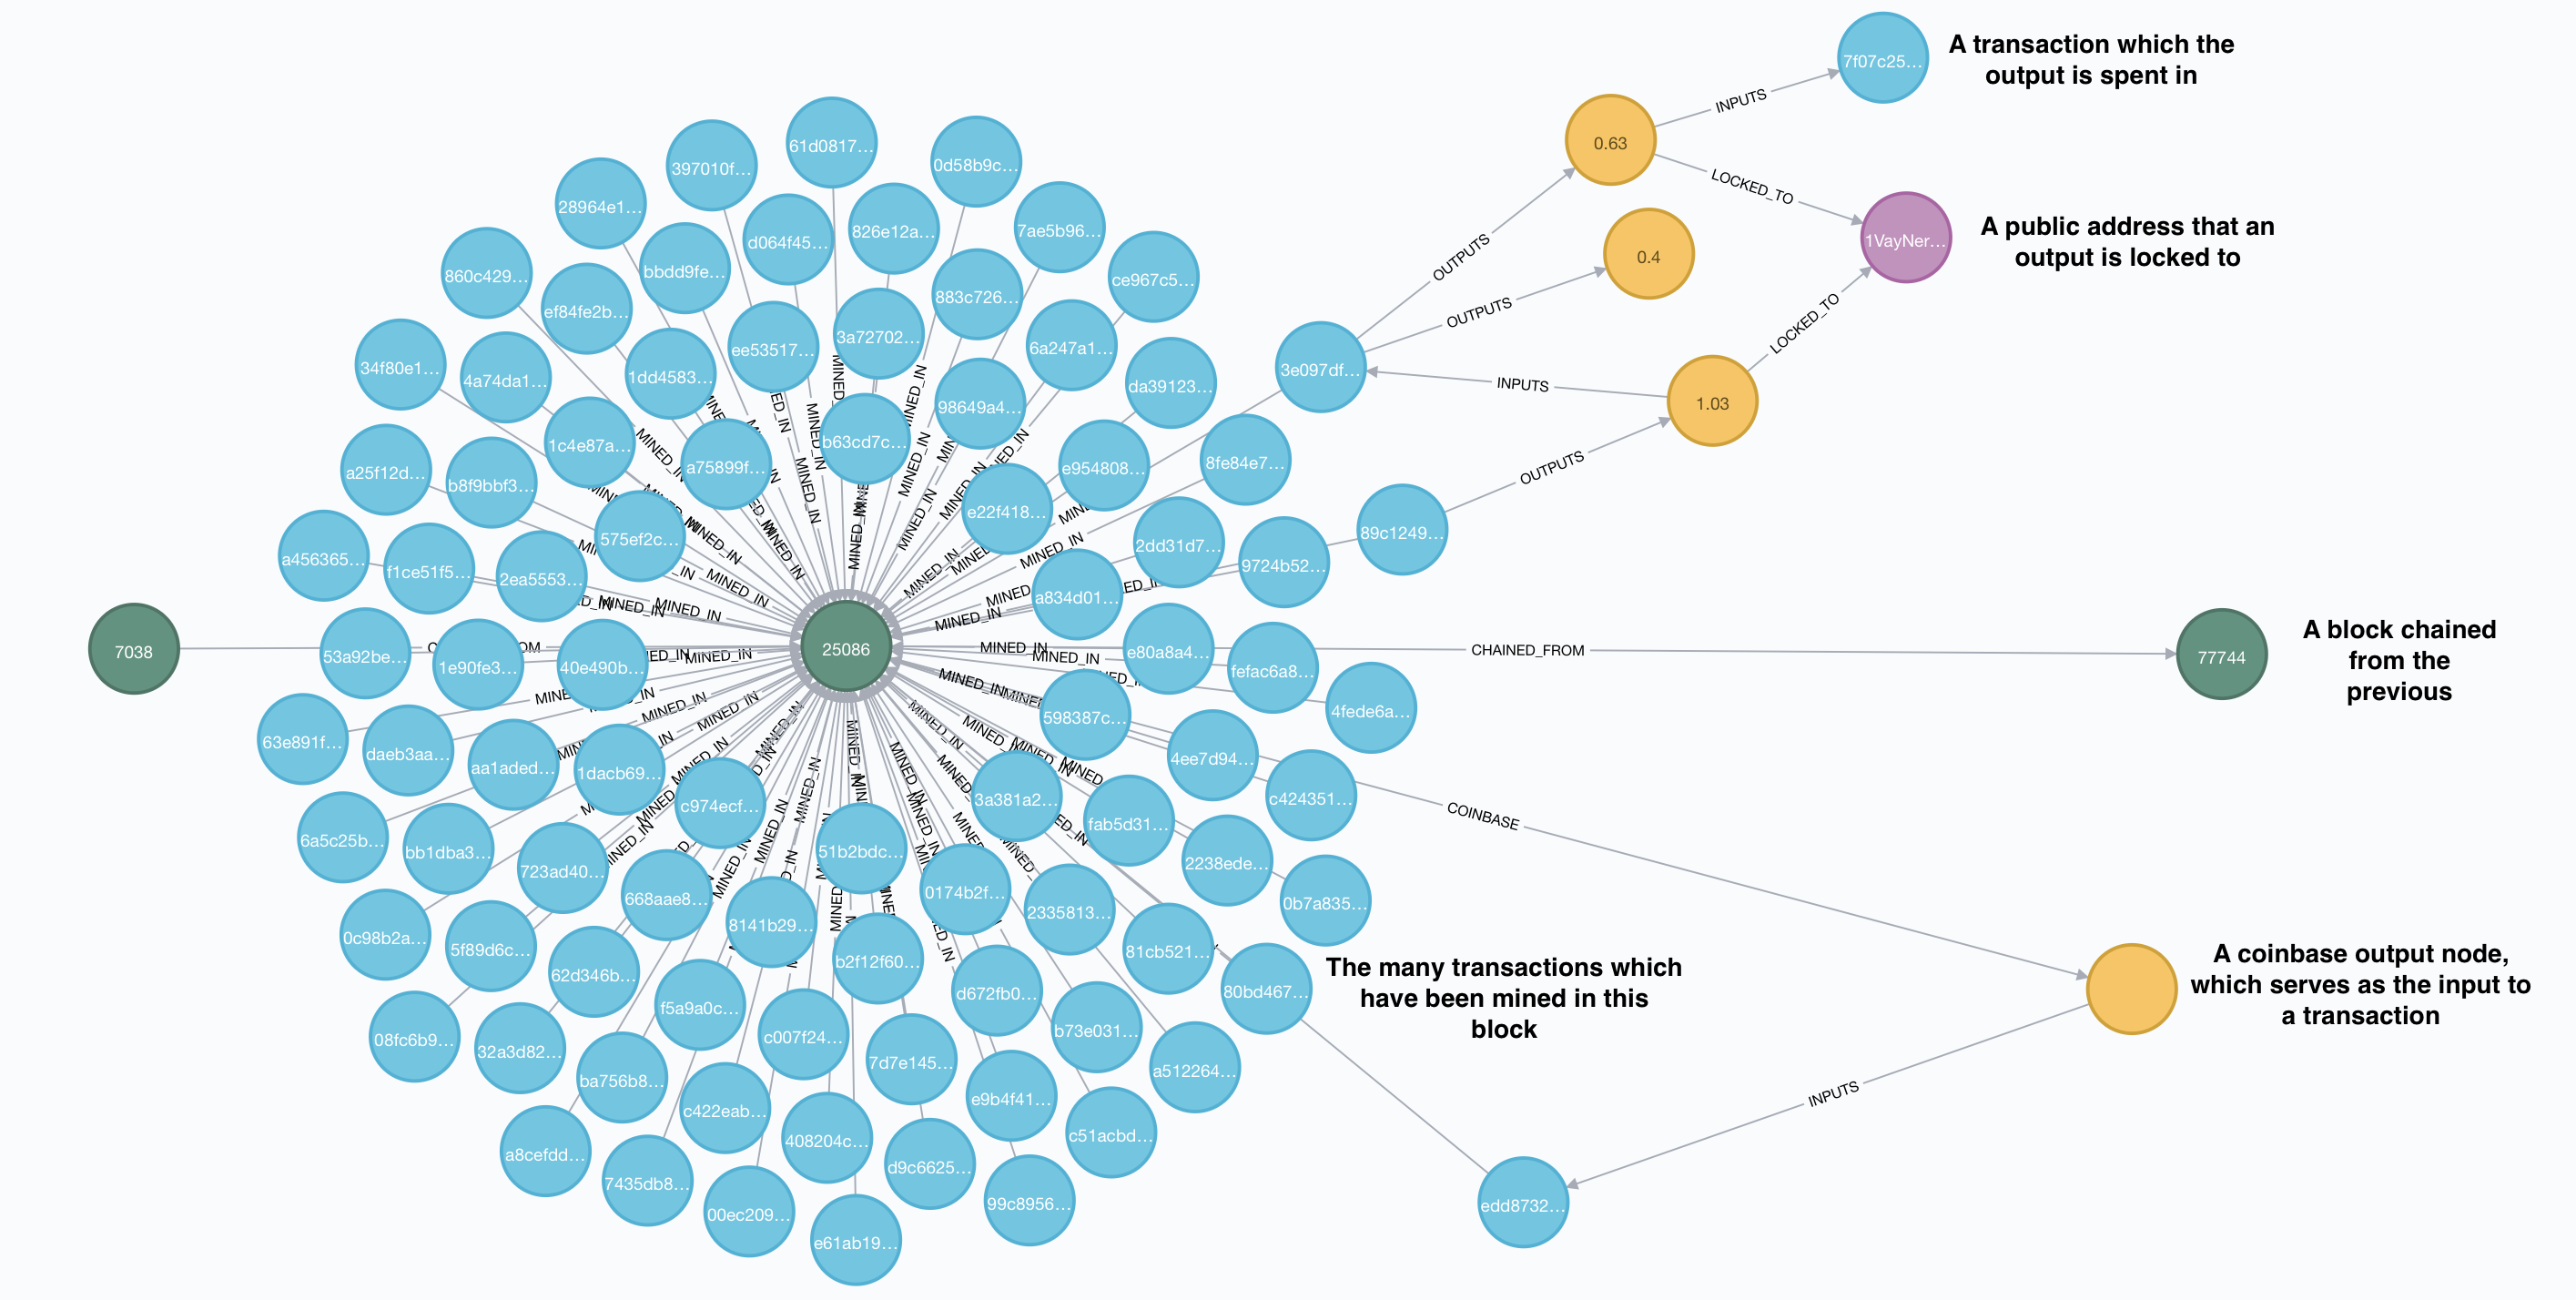
\includegraphics[width = 15cm]{./figures/neo4j-annotated}\\[0.5cm] 
  \caption{The nodes and relationships as visualised using the Neo4J Web UI}
  \label{fig:neo4j-layout}
\end{figure}

\subsection{Challenges \& Solutions:}
\subsubsection{Efficiency}
With multiple cores at my disposal, it would only be logical to try and distribute the workload across the cores. Fortunately, WebFlux conveniently provides functionality to do this; by adding \texttt{.parallel(n)} to my Flux stream, the workload is divided up into \texttt{n} rails. Then subsequently applying the \texttt{.runOn(Schedulers.parallel())} mapping, WebFlux is told to parallelise this work by running each rail on a separate core.  \todo{Some experimentatin figures for the speed up??}

\subsubsection{Job failure mitigation}
When an error from the client is received, possibly due to being overwhelmed with requests, it would be far from ideal for a single failure to cause the entire job to fail. Therefore I mitigated job failure by adding retry logic when requesting using the Reactive Client, so that failures will be handled by re-trying with a delay (the delay necessary to allow time for producer recovery in the case of being overwhelmed). Additionally, if an unexpected error occurs that I have not anticipated, the entire job may fail. Therefore, when performing the download, I ensured to do so in incremental batches. E.g I first download data for blocks 0-100,000 then 100,001-200,000 and so on. Therefore, if a failure does occur, progress from other blocks has been saved from successful runs and only the batch which failed needs to be re-run. 

\subsubsection{Writing concurrently from several threads}
Although the above parallelisation improves the efficiency of the overall download process, it introduced the problem of multiple threads writing to a single CSV file concurrently, which led to data in the CSV files being malformed where threads have written data chunks in an interleaving fashion. 
\\\\
\textbf{Fix interleaving writes with a lock:} Clearly each line in the file needs to be written atomically, so I introduced a lock that each thread must hold in order to perform a write to a CSV file. However, I quickly realised that this will create a significant bottleneck in the workflow and developed an alternative solution.
\\\\
\textbf{Fix interleaving writes with per thread files:} To enable parallel file writing and prevent the bottleneck of acquiring locks, I created a CSV file writer for each thread, for each data type. For example, the CSV file containing the block nodes will be named \texttt{block-data-thread-1.csv}, \texttt{block-data-thread-2.csv} and \texttt{block-data-thread-3.csv} etc. With this solution, each write can occur without risk of another thread also attempting to write, so the overhead of acquiring a lock for concurrent access is now redundant. \todo{Compare runs with and without}
\\\\

 
